\documentclass[a4paper,11pt]{article}
\usepackage[utf8]{inputenc}
\usepackage{fullpage}
\usepackage{graphicx}
\usepackage{wrapfig}
\usepackage{caption}
\usepackage{subcaption}
\usepackage{appendix}
\usepackage{tcolorbox}
\tcbuselibrary{theorems}

\newtcbtheorem[number within=section]{theo}{}%
{colback=green!5,colframe=green!35!black,fonttitle=\bfseries}{th}

\usepackage{hyperref}
\definecolor{navyblue}{rgb}{0.0, 0.0, 0.5}
\definecolor{myblue}{RGB}{15,77,145}
\definecolor{mountainmeadow}{rgb}{0.19, 0.73, 0.56}
\hypersetup{
	colorlinks=true,
	linkcolor=myblue,
	citecolor=mountainmeadow,
	urlcolor=navyblue,
}

\title{% 
	4F13: Probabilistic Machine Learning \\
	\vspace{10pt}
	\small Summarized from C. Rasmussen \& D. Krueger lectures, Michaelmas 2021}
\author{\small Oussama Chaib}
\date{\small October 2021}

\begin{document}
	\maketitle
	\tableofcontents
	\pagebreak
	\section{Prelude}
		\subsection{Machine learning: what and why?}
	\begin{itemize}
		\item Approach of the book: the best way to make machines that can learn from data is to use the tools of probabilistic theory.
		\item Probability theory: applied to anything involving uncertainties.
		\begin{itemize}
			\item What is the best prediction?
			\item What is the best model?
			\item What measurement should I perform next?
		\end{itemize}
		\item This systematic approach of using probability theory is often referred to as the \textbf{Bayesian approach}.
		\item To avoid upsetting some audiences, we use the more "neutral" term \textbf{probabilistic approach} (some of the methods we use like \textit{maximum likelihood} estimation are not Bayesian, but certainly fall under probabilistic methods).
		\item \textbf{Machine learning:} A set of methods that can automatically detect patterns in data, and then use them to predict future data or to perform other kinds of decision making using that data.
	\end{itemize}
	
	\subsection{Types of machine learning}
	\begin{enumerate}
		\item \textbf{Supervised (predictive):} Learn a mapping from inputs x to outputs y given a training set $D={(x_i,y_i)}_{i=1}^N$ containing N samples.
		\begin{enumerate}
			\item \textbf{Classification:} When the output $y_i$ is nominal (categorical) variable of a finite set (i.e: gender).
			\item \textbf{Regression:} When the output $y_i$ is real-valued.
		\end{enumerate}
		\item \textbf{Unsupervised (descriptive):} No specified pattern, no obvious error metric to use (i.e: neural networks).
		\item \textbf{Reinforcement learning:} Learning how to behave when given occasional reward or punishment signals.
	\end{enumerate}
	
	\subsection{Supervised learning}
	\subsubsection{Classification}
	\begin{itemize}
		\item Typical example: $y=f(x)$ with y is a \textbf{finite} number of points (x can be continuous, discrete, or a combination of both).
		\item We use the hat symbol to denote an estimate (i.e: $\hat{y}$ is an estimate of y).
		\item We would like to predict the result on novel input $x_*$, meaning ones that weren't seen before.
		\item \textbf{Probability notation:} Probability of output y given the input x, the training dataset D, and the model M.
		
		\item If the model is known and we do not wish to compare models, we drop the M so that: $p(y | x, D, M) \equiv p(y | x, D)$.
		\item Our best guess (most probable class label, mode of the distribution, MAP: maximum a posteriori estimate) will maximize this probability.
		\[
		\hat{y}=argmax^C_{c=1} \, \, (p(y | x, D, M)
		\]
	\end{itemize}
	
	\subsubsection{Regression}
	\begin{itemize}
		\item Just like classification but the response variable y is \textbf{continuous}.
		\item Will be explored further.
	\end{itemize}
	\subsection{Models for supervised learning}
	\begin{enumerate}
		\item \textbf{Parametric models:} $p(y | \mathbf{x})$ Fixed number of parameters. Usually faster but require \emph{stronger assumptions} about the nature of the data distribution.
		\item \textbf{Non-parametric models:} $p(\mathbf{x)}$ More flexible but computationally hungry for large datasets.
	\end{enumerate}
	\subsubsection{Linear regression}
	Can be written as follow:
	\[
	y(\mathbf{x}) = \mathbf{w^T}.\mathbf{x} + \epsilon
	\]
	where $\mathbf{w^T}$ is the vector containing \textbf{weights}, and $\epsilon$ the \textbf{residual error} (or noise) between our linear predictions and the input data.\\
	We often assume that the error vector follows a \textbf{Gaussian} or \textbf{normal} distribution:
	\[
	\epsilon \sim \mathcal{N}(\mu, \sigma^2)
	\]
	where $\mu$ is the \textbf{mean} and $\sigma^2$ the variance, and $\mathcal{N}$ represents the normal distribution. The parameters of the model can then be defined such that:
	\[
	\mathbf{\theta}=(\mathbf{w},\sigma^2)
	\]
	Linear regression can be used to model \textbf{non-linear} relationships by introducing a \textbf{basis function} $\mathbf{\Phi}(x)$:
	\[
	p(y | x,\theta) = \mathcal{N}(y| w^T\mathbf{\Phi}(x),\sigma^2) 
	\]
	\pagebreak
	\section{A brief review of probability theory}
	\begin{itemize}
		\item Probability of a union of two events:
		\[
		p(A \wedge B) = p(A) + p(B) - p(A \vee B)
		\]
		\item Joint probability:
		\[
		p(A,B) = p(A \vee B) = p(A | B)p(B)
		\]
		\item \textbf{Marginal distribution}: Rotating over all the possible values of another variable B. We write the joint probability of A and B as the product of a conditional probability and a marginal distribution.
		\[
		\underbrace{p(A,B)}_{joint\, probability} = \sum_{b} \underbrace{p(A | B=b)}_{conditional}\underbrace{p(B=b)}_{marginal}
		\]
		\item \textbf{Conditional probability}
		\[
		p(A|B) = \frac{p(A,B)}{p(B)}
		\]
		\item \textbf{Bayes rule}
		\[
		p(A|B) = \frac{p(B|A)p(A)}{p(B)}
		\]
		For practical cases:
		\[
		\underbrace{p(\theta|data)}_{posterior} = \frac{\overbrace{p(data|\theta)}^{\propto\,likelihood}\,\,\,\overbrace{p(\theta)}^{prior}}{p(data)}
		\]
		also:
		\[
		p(w|x,y,M) = \frac{p(w|M) p(y|x,w,M)}{p(y|x,M)}
		\]
		(x is removed in $p(w|M)$ because the weights $\mathbf{w}$ are independent of x)
		\item \textbf{Mean} (expected value) and \textbf{variance}
		\[
		\mu_X = E(X)=\sum_{\chi} x p(x) = \int_{\chi} x p(x)dx
		\]
		\[
		\sigma^2= var[X] = E[(X-\mu)^2]=\int (x-\mu)^2 p(x)dx
		\]
		\item \textbf{Gaussian (normal) distribution}
		\[
		\mathcal{N}(x|\mu, \sigma^2) = \frac{1}{\sqrt{2\pi\sigma^2}}\,\, e^{-\frac{1}{2\sigma^2} (x-\mu)^2}
		\]
		\item \textbf{Covariance:} Measures the degree of correlation between two random variables X and Y:
		\[
		cov[X,Y] = E((X-E(X)).(Y-E(Y))) = E(XY)-E(X)E(Y)
		\]
		Covariance can be between 0 and infinity. Correlation is normalized between -1 and 1.
		\item \textbf{Monte Carlo approximation}
		\[
		z = \int f(\chi)p(\chi)d\chi = \frac{1}{T} \sum_{s=1}^{S} f(x_s)	
		\]
	\end{itemize}
	\section{Introduction}
	\subsection{Modelling data}
	\subsubsection{Purpose of models}
	The purpose of models is:
	\begin{itemize}
		\item Making predictions
		\item Generalizing: interpolation, extrapolation
		\item Generating more data from a similar distribution as the training set
		\item Compressing and summarizing data
		\item Interpreting statistical relationships in data
		\item Evaluating the relative probability of a hypothesis on data
	\end{itemize}
	\subsubsection{Origin of models}
	The origin of models can be:
	\begin{itemize}
		\item \textbf{First principles:}  (i.e: Newtonian mechanics model, high level of accuracy)
		\item \textbf{Observations and data:} (i.e: annual production of timber depending on climate and geographical factors)
	\end{itemize}
	\textbf{Definition --} Machine learning is a broad term that covers theory and practice of mathematical models which to a significant degree rely on data.
	\subsubsection{Priors}
	Every model relies on priors: 
	\begin{itemize}
		\item \textbf{Knowledge}
		\item \textbf{Assumptions} (could be true or false)
		\item \textbf{Simplifying assumptions} (not necessarily true, but good enough -- i.e:  the mistake associated with the assumption is fairly small even though it might not be necessarily true)
	\end{itemize}
	\subsubsection{Components of a model}
	Time series have: 
	\begin{itemize}
		\item Unobserved/hidden/latent variables ($x(t)$, $x(t-1)$)
		\item Observations (shaded $y(t)$, $y(t-1)$)
		\item Parameters to link everything 
		\begin{itemize}
			\item Transitions (between latent variables)
			\item Emissions (from a lantent variable to an observation)
		\end{itemize}
	\end{itemize}
	\underline{\emph{Note:}} The number of latent variables increases with the number of observations, but the number of parameters doesn't!\\
	\textbf{-- Learning/training models:} "What to do with all this data?"\\ Depending on the data, some models include: inference, estimation, sampling, and marginalization.
	\subsubsection{Practical modelling}
	\begin{enumerate}
		\item Treat (training) the unobserved quantities (latent variables, observations, parameters)
		\item Make predictions based on test cases, interpret the trained model (can we figure out what the model is trying to tell us about the data?)
		\item Evaluate the accuracy of the data
		\item Model selection and criticism (choose the right model or variant of the model, identify limitations)
	\end{enumerate}
	There is not "true" or "correct" model -- \emph{"All models are wrong, but some are useful"} - George E.T. Box
	\subsection{Linear in the parameters regression}
	Let's start off with a dataset $D={x_i,y_i}^N_{i=1}$. From a dataset of N points, we would like to infer the coordinate $y_*$ at $x_*$. A simple model to do that would be polynomial \textbf{linear in the parameters} regression:
	\[f_w(x)=w_0+w_1 x+w_2 x^2+...+w_M x^M\]
	where $w_i$ are the corresponding weights of the polynomial, and the \textbf{parameters} of the model.
	\vspace{5pt}\\
	\textbf{-- Relevant questions:}
	\vspace{5pt}\\
	\emph{Model structure:} Should we choose a polynomial? What degree $M$ should we choose?\\
	\emph{Parameters:} What values of $w_i$ do we choose?
	\subsubsection{Least squares approach}
	Let's find the "best" polynomial (degree $M$ and weights $w_i$) according to the least squares approach (minimizing the variance or sum of squared error $e_i^2$):
	\[e_i(x)^2=(y_i(x_i)-f_w(x_i))^2\]
	\[E(x)=\sum^N_{i=1} e_i^2\]
	\vspace{5pt}\\
	\underline{\textbf{-- Some notations:}}
	\begin{itemize}
		\item \textbf{Training target} (input data that we would like to fit):
		\[  y = [y_1,...,y_N]  \]
		\item \textbf{Prediction} (the functions that will attempt to fit the data $y$):
		\[  f = [f_w(x_1),...,f_w(x_N)]  \]
		\item \textbf{Errors}:
		\[  e = f-y = [e_1,...,e_N]  \]
		\item \textbf{Parameters (what we're solving for!):} The \textbf{weights} of $f$:
		\[ w = [w_0,...,w_M]  \]
	\end{itemize}
	The sum of errors we would like to minimize is (defined as a variance to minimize):
	\[ E(w) = ||e||^2 = e^Te= (f-y)^T(f-y)\]	
	We define the \textbf{basis function} of the model (linear in the parameters model) as a matrix that contains all the $x^j$ (the matrix contains a list of all polynomials of unknown $x$ with maximum order from 0 to M) :
	\[ \Phi = \Phi_{i,j} =  \begin{bmatrix}
		\phi_0(x_1) & ... & \phi_M(x_1)\\
		... & ... & ...\\
		\phi_0(x_M) & ... & \phi_M(x_M)
	\end{bmatrix}
	\]
	\begin{center}
		where $\phi_j(x) = x^j $
	\end{center}
Ultimately, we can define the prediction function as a \textbf{linear in parameters} model that is the product of the \emph{basis function} and the \emph{weights}:
\begin{center}
	\fbox{$f = \Phi . w$}
\end{center}
To minimize the sum of squared errors $E(w)$, the gradient of the function should be equal to the zero vector:
\[  \frac{\partial E(w)}{\partial w} = 2 \Phi^T \Phi w - 2 \Phi^Ty = "0" \]
The weight vector $\hat{w}$ that minimizes $E(w)$:
\begin{center}
	\fbox{$\hat{w} = (\Phi^T Phi)^{-1} \Phi^T y$}
\end{center}
\textbf{The error vector is \underline{minimal} when it orthogonal with all columns of $\Phi$:}
\[ \Phi^T.e = 0 \]
\begin{figure}[h]
	\centering
	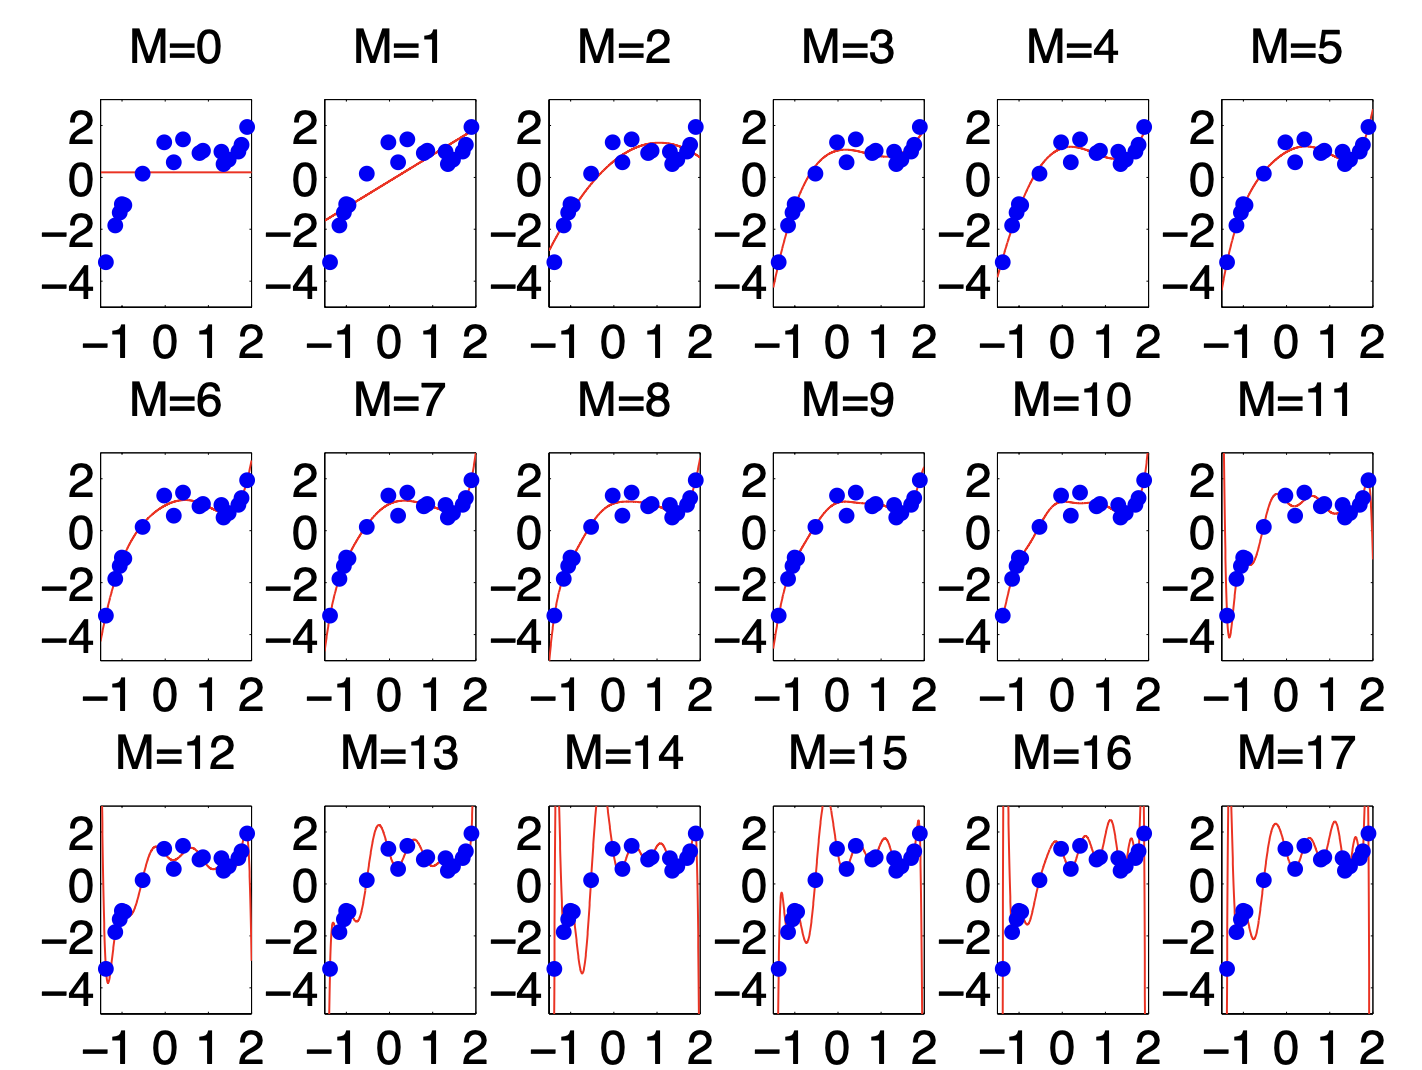
\includegraphics[width=.8\linewidth]{figures/M.png}
	\caption{Overfitting illustrated. In this example, we are solving for the \underline{weights} for each case of M}
\end{figure}
When we go to higher values of M, we are able to fit a function that minimizes the error term but we may run into the problem of \textbf{overfitting}. In that case, \textbf{additional assumptions} are needed.
\subsubsection{Probabilistic approach: Likelihood and concept of noise}
\textit{(Probabilistic view of what was done in the previous section. We're doing the exact same thing but using probabilities, only to end up getting equivalent weights)}\vspace{5pt}\\
\underline{\textbf{Definition:}} The \textbf{likelihood} is the probability of the data given the parameters.\vspace{5pt}\\
\textit{Example:}
\begin{itemize}
	\item $p(y|w,\sigma^2)$ is the probability of the observed data given the weights and noise.
	\item $L(w) \propto p(y|w,\sigma^2)$ is the \textbf{likelihood} of the weights.
\end{itemize}
The \textbf{maximum likelihood} of the weights:
\[ \hat{w} = argmax(L(w)) = argmax(e^{-\frac{E(w)}{2 \sigma_{noise}^2}}) = argmin(E(w)) \]
which is equivalent to the result that we got using least squares. But we still haven't solved the problem: we still overfit!
	\subsection{Comments from QnA}
	-- Why is the error vector $e$ minimal if it's orthogonal to all columns of $\phi$?\vspace{3pt}\\
	$\phi$ is a fixed function, it doesn't have any parameters in it. Still linear in parameters because the product of $w$ and $\phi$ matrices is linear (even at high polynomial orders).\vspace{5pt}\\
	-- What is Euclidian geometry?\vspace{3pt}\\
	Simple geometries, straight lines, basic shapes (including circle).\vspace{5pt}\\
	-- Bayesian methods, why are they not as popular?\vspace{3pt}\\
	Not so sure about that. Maximum likelihood (used often, single value that best explains the data, quite popular/successful).
	
\section{Bayesian inference}
Using Bayesian probabilities for statistical inference.  
\subsection{Maximum likelihood vs Marginal likelihood}
\begin{itemize}
	\item \textbf{Maximum likelihood}
	\begin{enumerate}
		\item Calculate the Gaussian likelihood:
		\[  p(y|x,w,M) = (\frac{1}{\sqrt{2\pi \sigma_{noise}^2}})^N \Pi_{n=1}^N e^{-\frac{(y_n-f_w(x_n))^2}{\sigma_{noise}^2}}\]
		\item Determine the weights $\mathbf{w}$ which maximize the likelihood \textbf{(maximum likelihood}:
		\[
		w_{ML}=argmax \, \, p(y|x,w,M)
		\]
		\item Make predictions!
		\[
		p(y_*|x_*,w_{ML},M)
		\]
	\end{enumerate}
	\item \textbf{Marginal likelihood} (or "evidence")
	\begin{enumerate}
		\item Calculate the marginal likelihood:
		\[
		p(y|x,M)=\sum p(w|x,M)\,\overbrace{p(y|x,w,M)}^{likelihood}dw = \mathcal{N}(w;\mu,\Sigma)
		\]		
		\textbf{\underline{Depends ONLY on your training sets and model}}\\
		\item Find the point where \[log(marginal\,likelihood) = 0\]
		\item Make predictions:
		\[
		p(y_*|x_*,x,y,M)=\int p(y_*,w|x_*,x,y,M)dw = \int p(y_*|w,x_*,M)\,p(w|x,y,M)dW
		\]
		\begin{figure}[h]
			\centering
			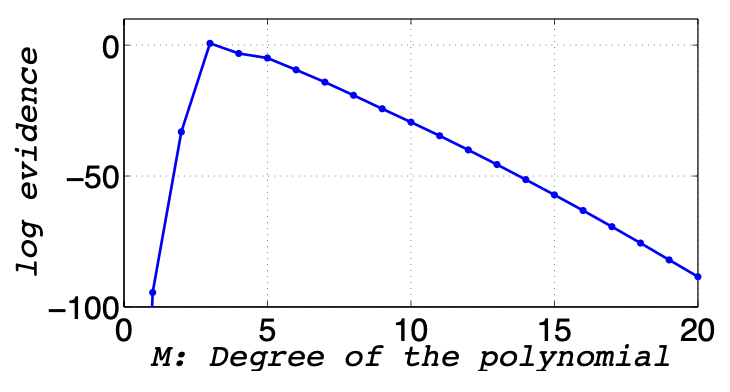
\includegraphics[width=.5\linewidth]{figures/razor.png}
		\end{figure}
	\end{enumerate}

\end{itemize}
How can probabilities be higher than 1? Not the case for \textbf{probability densities}.
\end{document}